\subsubsection{\texttt{RF-7}: compartición de código asociado a un curso}
\label{subsec:rf7}

Existen dos formas para hacer que un estudiante quede matriculado en un curso, tanto en la extensión como en la aplicación web: puede ser inscrito manualmente por un profesor (\referenciaConTT{subsec:rf6}{RF-6}) o puede automatricularse (\referenciaConTT{subsec:rf8}{RF-8}), que requiere de un código que deben ser proporcionado por el docente.

La extensión permite a los docentes obtener un enlace al servidor de \textit{VSCode4Teaching} en uso que puede divulgar al estudiantado que desee que se automatricule. Este enlace incluye un código único que identifica biunívocamente cada curso existente en la plataforma. Para generarlo, la visualización de los cursos para docentes (\referenciaConTT{subsec:rf1}{RF-1.2}) dispone de un botón ``Share with students'' (compartir con estudiantes) que, tal como queda plasmado en la \referenciaFigura{fig:reqf7-1}, muestra a los docentes el código único para la automatrícula en el curso como, además, el enlace al servidor que los alumnos pueden abrir en el navegador para consultar información adaptada al caso del curso específicamente divulgado, incluyendo instrucciones acerca de cómo inscribirse en el curso compartido.

\begin{figure}[ht]
    \centering
    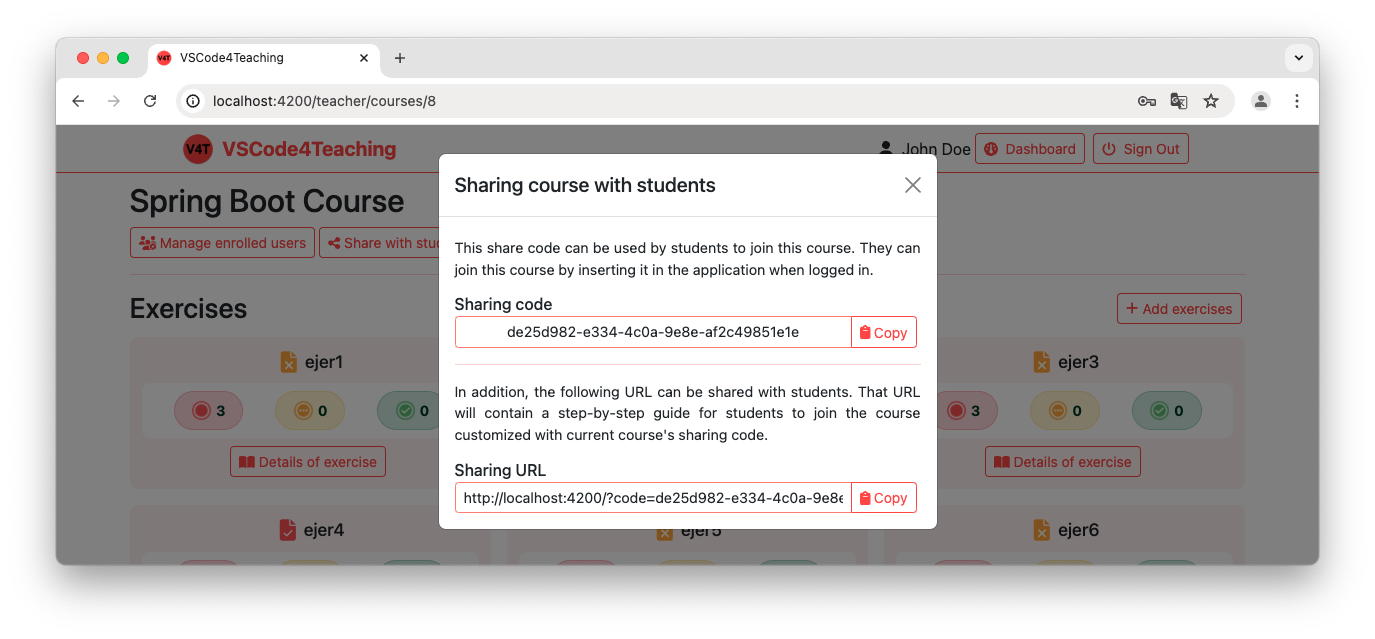
\includegraphics[width=\textwidth]{imagenes/utilizadas/4-3-implementacion/rf7-1.png}
    \caption{Información para la compartición del código único de automatrícula en un curso.}
    \label{fig:reqf7-1}
\end{figure}
